
\documentclass[12pt]{article}
\usepackage[utf8]{inputenc}
\usepackage{amsmath}
\usepackage{graphicx}
\usepackage{listings}
\setlength{\parskip}{\baselineskip}%
\setlength{\parindent}{0pt}%

\title{Computational Complexity Assignment 1}

\author{Tyler Tracy}

\begin{document}

\maketitle


\section{Problem 1}


The goal of this turing machine is to use a 3 tape turing machine to detect if a string is a palindrome.

My basic approach was to reverse the input string onto the second tape and then compare the first and second tape to see if they are the same.

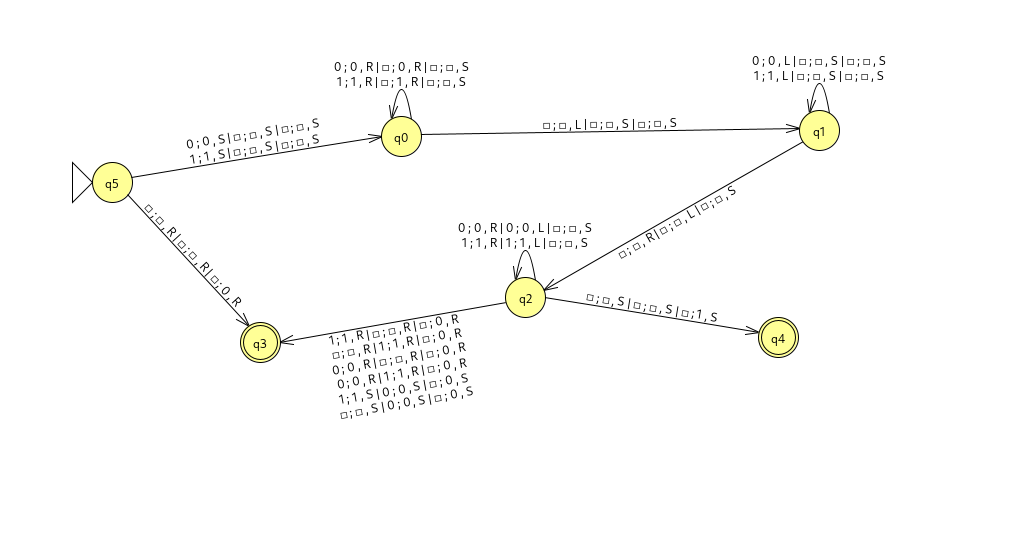
\includegraphics[width=\textwidth]{problem1.png}

Below I provide pseudocode for the turing machine and an analysis of the time complexity of each line

\begin{lstlisting}[basicstyle=\small, tabsize=3]
# Check for empty strings
If symbol under the first head is empty then halt # O(1)
# Move the head to the end of the input,
# Copying the string to the second tape
While first head is under a non-empty symbol # O(n)
	Move first head right # O(1)
	Write the symbol under the first head to the second tape # O(1)

# Move the first head back
While first head is under a non-empty symbol # O(n)
	Move the first head left # O(1)

# Compare the two strings
While first head is under a non-empty symbol # O(n)
	If the symbol under the first head is not the same
	as the symbol under the second head then halt # O(1)
	Move the first head right # O(1)
	Move the second head left # O(1)
\end{lstlisting}

Adding all these complexities up and dropping the constants we get O(n) for the time complexity of the turing machine.


\section{Problem 2}
The purpose of this turing machine is to detect if a string is a palindrome using a single tape turing machine.

My basic approach was to go back and forth between the beginning and end of the string and compare the characters at each end. If they are every different then the string is not a palindrome.

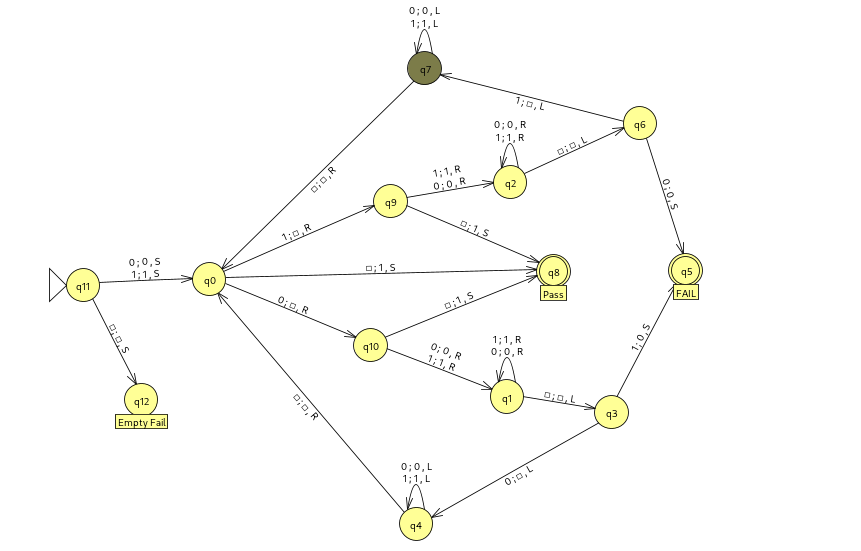
\includegraphics[width=\textwidth]{problem2.png}

Below I provide pseudocode for the turing machine and an analysis of the time complexity of each line

\begin{lstlisting}[basicstyle=\small, tabsize=2]
# Check for empty strings
If symbol under the head is empty then halt # O(1)

Store the symbol under the head in a variable i # O(1)
Erase the symbol under the head # O(1)

While the head is under a non-empty symbol # O(n)

	# Move the head to the end of the input # O(n)
	While head is under a non-empty symbol # O(n)
		Move head right # O(1)
	Move the head left # O(1)

	If the symbol under the head is not the same as i
		then halt # O(1)

	# Move the head back to the beginning of the input
	While head is under a non-empty symbol # O(n)
		Move head left # O(1)
	Move head right # O(1)
\end{lstlisting}







\section{Problem 3}

My python program reads the .jff file that is made by jflap to encode a turing machine. JFLAP uses xml to encode the turing machine. XML is not the most space efficient way to encode something, but it is very robust and readable. The only part of the jff file that I use is the part that encodes the transitions and the part that labels the states. From the transitions, the tape alphabet and the input alphabet can be derived from all the symbols that appear. Since XML can encode an arbitrary number of elements, this format can encode any turing machine.





\end{document}